\chapter{三点估算} % Introduction chapter suppressed from the table of contents

\hypertarget{ux4f30ux7b97ux662fux4e00ux4e2aux8303ux56f4ux4e0dux662fux4e00ux4e2aux6570}{%
\subsection{估算是一个范围,不是一个数}\label{ux4f30ux7b97ux662fux4e00ux4e2aux8303ux56f4ux4e0dux662fux4e00ux4e2aux6570}}

唐工:你估计要完成开发用户登录模块要多少天?\\
小李:三天。\\
唐工:能在三天完成的可能性有多高?\\
小李:可能性很高。\\
唐工:可否量化一点?\\
小李:可能性为50\%-60\%。\\
唐工:所以很有可能不止三天,要四天了。\\
小李:对的,其实也有可能要五、六天,但我估计机会不大。\\
唐工:你信心有多少?\\
小李:难说,有95\%的信心可以在六天之内完成。\\
唐工:所以有可能要用上七天了?\\
小李:这样说吧,如果所有可能出问题的都出了问题,甚至会10天或11天,但这种概率很低。\\
(最终管理者唐工还是要求有一个承诺,而不是一个估算)\\
所以唐工再问小李:是能否给我一个确实能完成这个模块的日期?\\
小李:正如我前面说,很可能三天可以完成,但有可能四天。\\
唐工追问:你可以说四天吗?\\
小李:也有可能五六天。\\
唐工结束对话:OK,请你尽力六天之内完成这个模块。\\
唐工貌似请求,但实际是要求小李承诺这个模块要在六天之内开发完。假如这个模块的开发时间超过六天,唐工就有依据说小李没有尽力导致延误了。\\
所以从以上对话,可以看到作为开发专业人员,必须分清估算和承诺。作为专业人士,我们不应该给一些没有把握的承诺,误导对方。中国老话说一诺千金就是这个道理。

\hypertarget{ux4eceux5355ux70b9ux5230ux4e09ux70b9ux4f30ux7b97}{%
\subsection{从单点到三点估算}\label{ux4eceux5355ux70b9ux5230ux4e09ux70b9ux4f30ux7b97}}

从上面的例子可以看到,一般的单点估算是很容易被误导,以为那个天数是有把握达成的,所以我们最好从单点估算变成三点估算,除了估算最可能的天数,还有最佳和最差共三点。但项目是由一系列的任务组成(如第二任务依赖于第一个任务的完成),如何计算所有任务的总天数?
下面用例子说明如何用3种使用3点估算估计的方法(A、B、C)估算总天数:\\
A)假定都是正态分布,用模型估计:\\
先用PERT方程式计算每一步的预计值 与 标准差:\\
::预计值 Expected Value EV = (Best + 4xMost Likely + Worst ) /6\\
::标准差 Sigma= (Worst - Best) / 6\\

%Screenshotfrom2023-11-1221-23-06.png

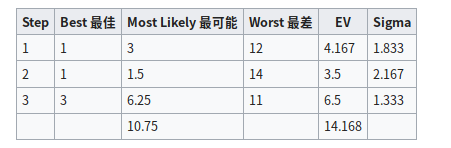
\includegraphics[width=6cm]{Screenshotfrom2023-11-1221-23-06.png}

如果假定是正态分布,按以上预计值和标准差,使用蒙特卡洛模拟,从下图可看到,95\%范围是
8.02 \textasciitilde{} 20.37\\
%\url{文件:pert3.1.png}

\includegraphics[width=6cm]{pert31.png}

B) 直接用PERT方程式计算总天数的均值与标准差:\\
如不用模拟,直接把3步的均值加起来\\
::4.2 + 3.5 + 3.6 = 14\\
计算3步总方差:(方差 = \(Sigma^2\))\\
假定: 总方差 = 每步方差的总和\\
总方差 = 9.77\\
Sigma \(\sigma\)= 3.13\\
95\%范围计算公式为:均值的总和
\(\pm 2 \sigma = (4.2 + 3.5 + 3.6) \pm 2 x 3.13  = 14 \pm 6.26\)= 7.74
\textasciitilde{} 20.26\\
结果与蒙特卡洛模拟预测类似。\\
C) 假定都是三角形分布,用模型估计:\\
如果用三角形分布,95\%范围是 10.38 \textasciitilde{} 26.45\\
%\url{文件:pert32.png}

\includegraphics[width=6cm]{pert32.png}

\hypertarget{ux603bux7ed3-ux89e3ux8bfbux5206ux6790ux7ed3ux679c}{%
\subsection{总结 +
解读分析结果}\label{ux603bux7ed3-ux89e3ux8bfbux5206ux6790ux7ed3ux679c}}

\begin{itemize}
\tightlist
\item
  如果假定每一步的分布都是一个正态分布,就可以用头两个方程式计算每一步的平均值跟标准差和方差,用方程式可计算3步的总均值大概是14。也可以用方程式计算标准差,总的sigma
  (标准差)是3.13左右。
\item
  也可用蒙特卡洛模型(假定步骤都是正态分布),得出很类似的正态分布,总的平均也接近14,95\%的范围是从8.02到20.37,
  接近上面算出的均值 \(\pm\) 两个标准差数值。
\item
  但因三个步骤都是明显往右偏,所以不能假设它们是正态分布,更合适的是使用三角形分布,然后用蒙特卡洛估算``加''起来的分布,看见最后一个图明显是类似往右有个尾巴,能更正确反应三个步骤加起来的天数的估计分布。
\item
  跟假定正态分布的结果比较,很明显看到用三角形分布结果往右偏,上限是
  26.45(比正态分布的20.37
  高)。不是正态分布的话,左面就没有长尾巴,所以就会比本来正态分布的下限高,下限是
  10.38 (比正态分布的 8 高)。
\item
  从这简单例子看到,如果我们要把三点估算加起来,尤其是非正态分布的话,就不能用简单的方程式,或者假定它是正态分布来计算,需要用蒙特卡洛模型假设三角形分布才能真正反应总体的分布。\\
\end{itemize}

从这三个偏左分布步骤例子看起来好像有些偏差,但不是很严重。如果我们看见用十个步骤都是偏一边分布,总分布会如何?是否相差会更远?

\hypertarget{ux5229ux7528ux8499ux7279ux5361ux6d1bux6a21ux62df10ux4e2aux6b65ux9aa4ux4e09ux89d2ux5f62ux5206ux5e03ux7684ux603bux5206ux5e03}{%
\subsection{利用蒙特卡洛模拟10个步骤(三角形分布)的总分布}\label{ux5229ux7528ux8499ux7279ux5361ux6d1bux6a21ux62df10ux4e2aux6b65ux9aa4ux4e09ux89d2ux5f62ux5206ux5e03ux7684ux603bux5206ux5e03}}

如果每步都估算天数,10个步骤的 总天数就是500天 (把10个估算值加起来)。

但如果每个步骤都是三点估算:

%Screenshotfrom2023-11-1221-25-44.png

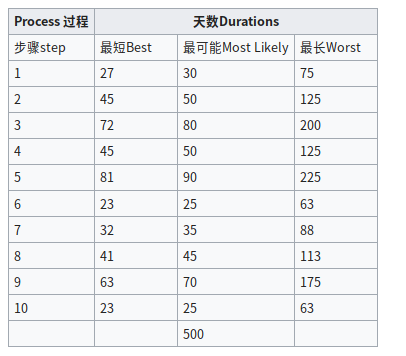
\includegraphics[width=6cm]{Screenshotfrom2023-11-1403-10-17.png}

很明显看到每一步都是偏左的分布,所以可预计总天数应不止500天,
但估多少才合适?

假定每步骤是三角形分布,用模型估计,重复五千次,得出下面分布:

%\href{文件:HMTT_v1.3_s77.png}{400px}

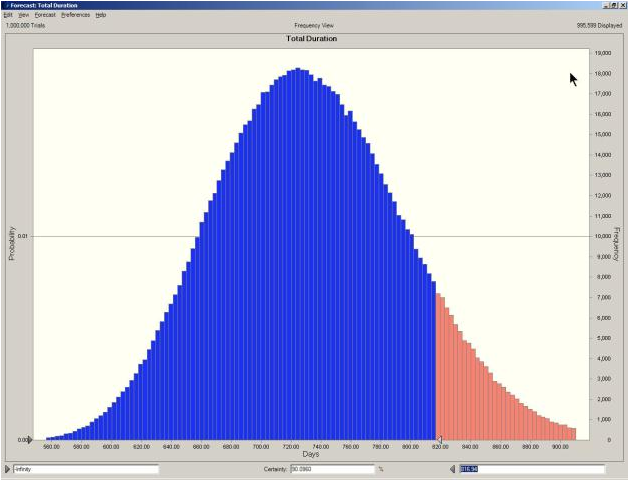
\includegraphics[width=6cm]{HMTT_v13_s77.png}

%Screenshotfrom2023-11-1221-27-17.png

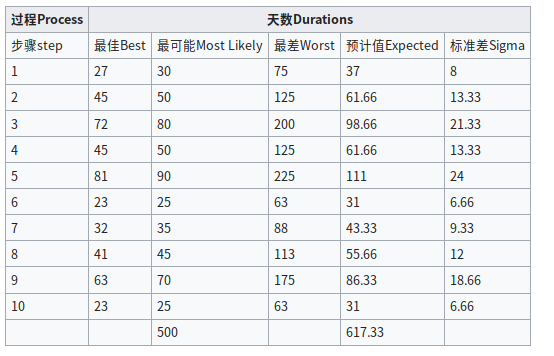
\includegraphics[width=6cm]{Screenshotfrom2023-11-1403-10-57.png}

A) 用PERT方程式计算每一步的预计值 与 标准差:

%\href{文件:10stepsPertScreenshot_2022-10-24_205007.jpg}{500px}

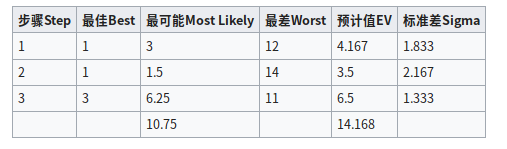
\includegraphics[width=6cm]{Screenshotfrom2023-11-1403-12-52.png}

假定是正态分布,按以上预计值和标准差,使用蒙特卡洛模拟,得出的总分布与上面用三角形分布的结果几乎一致,都是左右平均分布的正态形。

\hypertarget{ux5206ux679010ux6b65ux9aa4ux6a21ux62dfux7ed3ux679c}{%
\subsection{分析10步骤模拟结果}\label{ux5206ux679010ux6b65ux9aa4ux6a21ux62dfux7ed3ux679c}}

\begin{itemize}
\tightlist
\item
  为什么用三角形模拟出来不是偏左的分布(类似前面3步结果),而是一个正态分布
\end{itemize}

\begin{description}
\tightlist
\item[]
以上实验验证了``中心极限定理'',无论本来是什么形状的分布,如果随机抽样够多,样本的平均值分布接近正态分布。所以如果本来只是3个步骤的时候还是可以看出是三角形偏左,但到了用十个步骤相加的时候,就跟每个都是用正态分布去估算的结果没有什么区分。\\

(中心极限定理会在后面数据分析里用上,例如通过画控制图判断过程是否稳定)\\
\end{description}

\begin{itemize}
\tightlist
\item
  实验结果也验证了PERT三点估算法公式,无论任何分布都可以用PERT公式计算每一步的预计值和标准差,然后计算总结果的分布(不需要蒙特卡洛模拟),当步骤越多差异就越小,如果是像上面的例子,只是希望求10个步骤的总分布(无论每步本身是怎样分布),都不需要用模拟,用PERT公式计算便可。\\
\end{itemize}

\begin{description}
\tightlist
\item[]
(这不表示蒙特卡洛模型没有用,到后面根因分析部分,我们还是会继续用它来比较不同的搭配选择最优)
\end{description}

\hypertarget{ux9644ux4ef6}{%
\section{附件}\label{ux9644ux4ef6}}

\hypertarget{ux8499ux7279ux5361ux6d1bmonte-carlo-ux6a21ux62df}{%
\subsection{蒙特卡洛(Monte Carlo)
模拟}\label{ux8499ux7279ux5361ux6d1bmonte-carlo-ux6a21ux62df}}

当结果不能用数学公式计算的时候(例如是三角形分布),可以用电脑随机模拟结果。例如:

\begin{itemize}
\tightlist
\item
  计算3个步骤的总共人天,每个步骤都是三角形分布,我们就用电脑的随机功能模拟,让随机功能的结果按三角形分布:
\item
  第一次模拟:步骤1得出1.3,步骤2得出1.2,步骤3得出2.0,得出三个步骤的总工期是4.5人天。
\item
  第二次......。
\item
  如果我们模拟1000次,10000次就有,便能模拟出总分布。
\end{itemize}

5000次

%\href{文件:捕获2-1.PNG}{500px}

%\href{文件:捕获2.PNG}{500px}

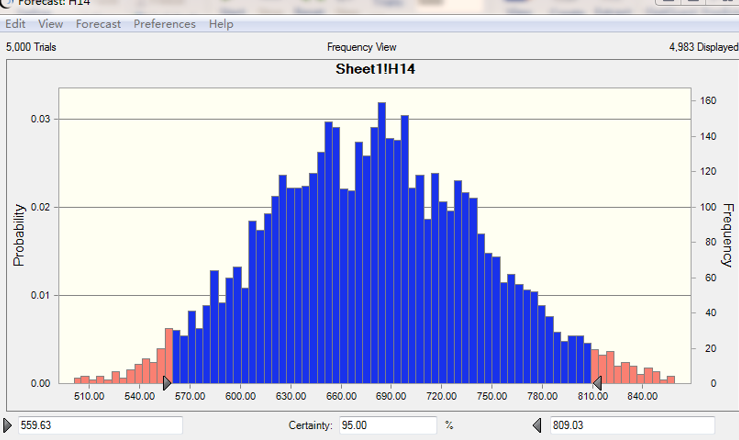
\includegraphics[width=6cm]{捕获2-1.PNG}

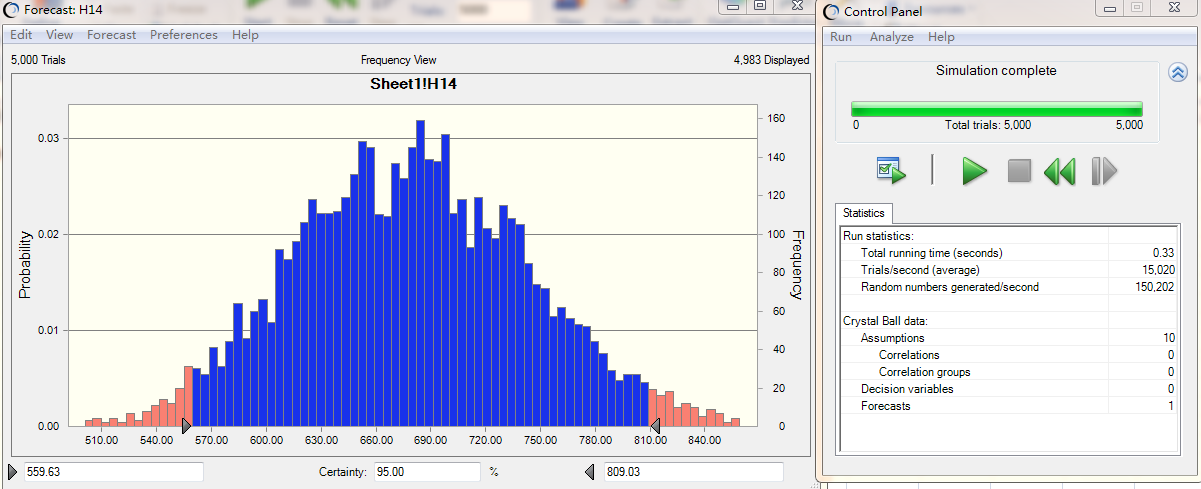
\includegraphics[width=6cm]{捕获2.PNG}

10000次

%\href{文件:捕获1-1.PNG}{500px}

%\href{文件:捕获1.PNG}{500px}

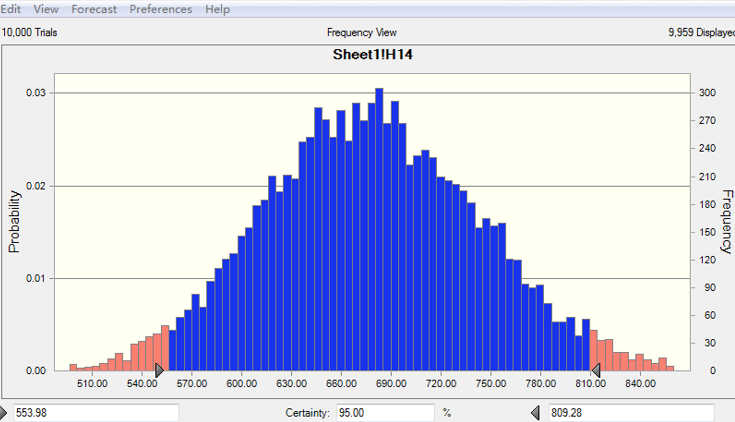
\includegraphics[width=6cm]{捕获1-1.PNG}

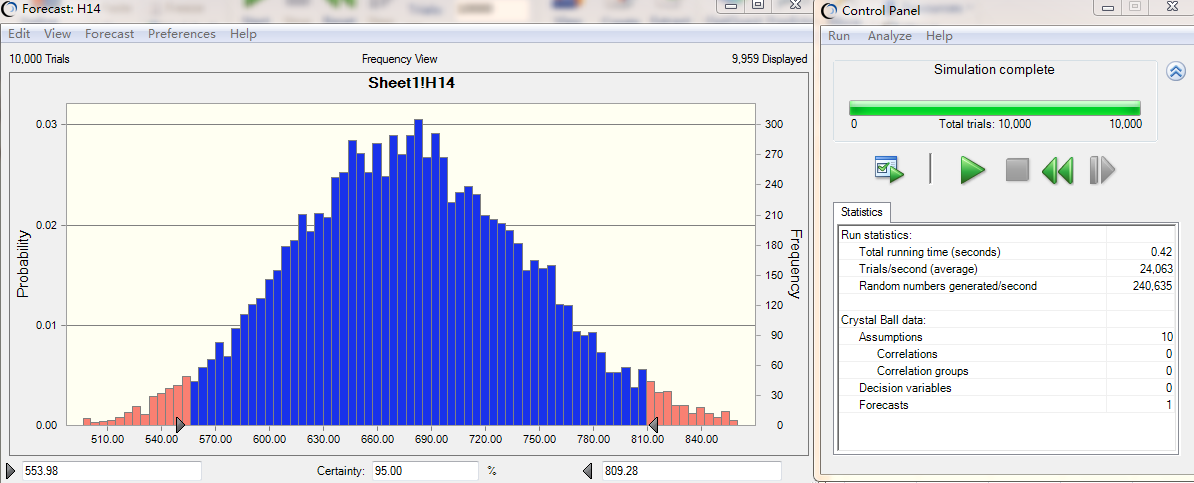
\includegraphics[width=6cm]{捕获1.PNG}


